% What is MIxT used for? And how would users do it in VR?
% How the MIxT application is implemented in GeneNet VR and what it does.
% What are typical network characteristics for this (type of) application? Size, clusters, edges, connectivity, etc?

We have implemented MIxT in GeneNet VR as a case study in order to work with realistic and large biological networks. In addition, we used this in the evaluation since it is a realistic application where we used complex networks that originally didn't scale in the existing web application \footnote{https://mixt-tumor-stroma.bci.mcgill.ca/network}.
In this chapter we will talk about what MIxT is used for, its disadvantages for scaling large biological networks and the challenges of building a VR visualization system for these type of networks.

\section{What is MIxT used for?}
MIxT blood-tumor is a web application for interactive data exploration in system biology developed by UiT and Concordia University\cite{fjukstad_dumeaux_olsen_lund_hallett_bongo_2017}. In addition, a reasearch was carried out for the study of interactions between the tumor and the blood systemic response of breast cancer patients\cite{dumeaux_fjukstad_interactions_tumor_blood}. In the study, they profiled RNA in blood and matched tumor from 173 patients with breast cancer. The goal of the study was to identify genes and pathways in the primary tumor that are tightly linked to genes and pathways in the patient's systemic response (SR). The SR is the body's response to an infectious or non-infectious insult. A biological pathway is a series of actions among the molecules in a cell that leads to a certain product or change in the cell. The result of the study suggests new ways of monitor breast cancer by looking outside the tumor and studying the patient's systemic response.

[Explain Figure and write about the different modules and biological prorcesses]

\begin{figure}[h!]
    \setlength{\tempheight}{15ex}
    \centering
    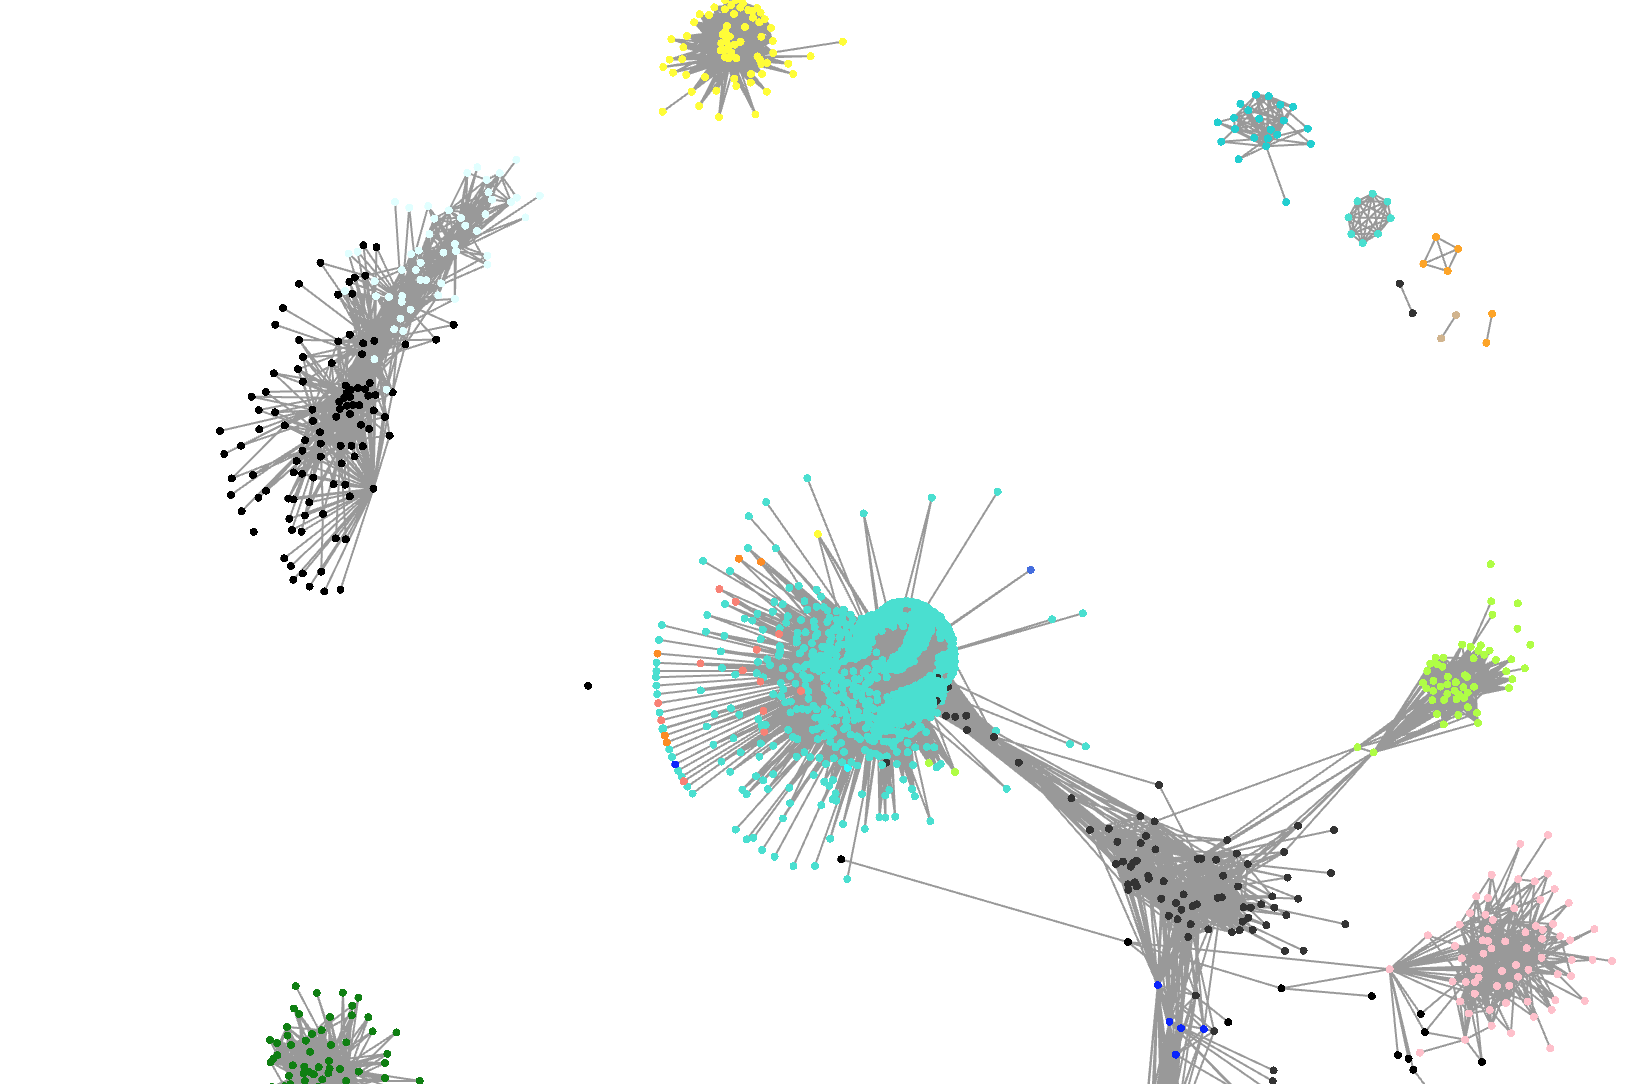
\includegraphics[width=\textwidth]{mixt_webapp}
    \caption{Screenshot from the network visualization in the MIxT web application. The system is 2-dimensional and the user can zoom in and out in the network. It is also possible to hover on a node to see its name.}
    \label{fig:mixt_webapp}
\end{figure}

\section{MIxT in VR}
MIxT is originally a 2-dimensional visualization system that is used in the browser. When working with a VR version of MIxT we had to take into account several aspects. In the first place, we have a new dimension in the visualization system, since it's 3-dimensional. In the second place, we don't have the limitations that a browser usually has; the limitation depends now on the hardware from the machine or the Oculus Quest. Finally, VR offers a lot more interaction possibilities than we can find in a browser, this is thanks to the controllers.

Adding a new dimension offered a new way of visualizing the datasets in MIxT. We could now see the network from any angle. Also, with VR, we also have the immersion feeling that otherwise is hard to have in a 2-dimensional screen.

[Continue writing about hardware and interactivity in VR]

\section{Network characteristics}
The human being has 23 pairs of chromosomes in each of our cells. Each chromosome can contain from hundreds to thousands of genes. There are estimated to be around 30.000 genes. In GeneNet VR, the blood dataset is the biggest one, and contains a total of 2693 genes. We don't expect to deal with a network of 30.000, but it is true, as we can see from the datasets, that they can contain several thousands nodes and also several thousand edges. For instance, in the blood dataset, we can find a node that has 1607 relationships to other nodes.

[What are typical network characteristics for this (type of) application? Size, clusters, edges, connectivity, etc?]
